%The Materials and Methods section provides sufficient detail for other 
%scientists to reproduce the experiments presented in the paper. In some 
%journals, this information is placed in an appendix, because it is not what 
%most readers want to know first.

% explicit preview would be phrased much like the object of the document: 
%"This section first . . . , then . . . , and finally . . . "
% Do not make readers guess: Make sure the paragraph's first sentence gives 
%them a clear idea of what the entire paragraph is about.
%%%%%%%%%%%%%%%%%%%%%%%%%%%%%%%%%%%%%%%%%%%%%%%%%%%%%%%%%%%%%%%%%%%%%%%%%%%%%%
\section{Adaptive Optics Methods applied in Microscopy}
\label{sec:ExperimentDiscussion}

Adaptive optics techniques have found their way into almost all kinds of modern, high resolution microscopy techniques. These microscopes have been combined with direct wavefront sensing and sensorless AO, using deformable mirrors or spatial light modulators for aberration compensation~(all of which have been described in Section~\ref{Measurement}. This includes standard widefield microscopes as well as highly sophisticated and specialized point scanning methods such as CARS and Stimulated Emission Depletion~(STED) techniques. It has to be noted however, that some of these methods are themselves only a few years old. Therefore, they are still being optimized and so are the AOM techniques. It is an interesting field of research with new ideas being implemented every year.

AO was first used in confocal and two-photon fluorescence microscopy, both of which are commonly used in biomedical applications. These microscopes suffer from a significant drop in signal and resolution as the focus is moved deeper into the specimen, which is caused by aberrations~\cite{characterizing_abberations}.

AOM is also used for imaging of live specimens. Due to an increased excitation signal and improved light collection from the specimen, acquisition times can be reduced and contrast can be enhanced. Techniques that without AO are too slow for live imaging might now be usable, opening up completely new fields of research. Another advantage of AO lies in the microscopy design. Using AO methods, can help the designer to relax the aberration tolerance. This permits a significant reduction in the complexity of the optical system while maintaining diffraction limited operation.

This section will describe, using state of the art examples and how AO is implemented in both widefield and point scanning systems.  


%%%%%%%%%%%%%%%%%%%%%%%%%%%%%%%%%%%%%%%%%%%%%%%%%%%%%%%%%%%%%%%%%%%%%%%%%%%%%
\subsection{Widefield Microscopy}
\label{sec:WidefieldMicroscopy}

As mentioned above, AO techniques are being applied in widefield microscopy. In conventional microscopes, widefield illumination is provided using back light illumination or in the case of reflection or fluorescence modes, via the objective lens. The image quality depends only on the aberrations induced in the detection path and is independent of the aberrations of the illumination path. Aberration correction is therefore only necessary in the detection path and a single pass adaptive optics system will suffice~\cite{book_aberrations}. Hence, the goal of AO for widefield microscopy is to restore the best possible imaging and to correct for aberrations induced both by an imperfect imaging system as well as by the imaged specimen. The latter becomes more important for thick biological samples where the light has to travel a larger distance through a medium with an inhomogeneous refractive index. 

Many other highly specialized widefield microscopy techniques have been developed and for most of those, AO schemes for aberration correction and resolution optimization have been presented. Three widefield microscopy techniques will be presented in this section, starting with the implementation of direct wavefront sensing for a fluorescence microscope in ~(Section~\ref{sec:DirectFluorescenceMicroscope}). The implementation of AO in a standard transmission microscope using a sensorless wavefront sensing scheme is explained in~(Section~\ref{sec:TransmissionMicroscope}) and finally, how the theoretical background of this technique can be applied to more sophisticated microscopy schemes is then shown on the example of structured light illumination~(Section~\ref{sec:StructuredIlluminationMicroscopy}), a specialized wide field technique. 

%For fluorescence microscopy, the aberration caused by an refractive index mismatch between sample, cover plate and immersion medium can by calculated theoretically and is then corrected~\cite{wide_AOM_FM_spehrical_correction} or the aberration is measured using a guide-start technique~\cite{wide_fluorescence_guide_star} as described in Section~\ref{Measurement}. Since the techniques applied in fluorescence microscopy are very similar to the ones presented for transmission microscopes, they will not be explicitly covered here. AO is also applicable in multifocal multiphoton microscopy~\cite{wide_MPFM,wide_MMM_AO}.%

%------------------------------------------------------------------------------
\subsubsection{Direct Wavefront Sensing in a Fluorescence Microscope}
\label{sec:DirectFluorescenceMicroscope}

While indirect sensing has several advantages over direct sensing~(see sec. \ref{sec:IndirectWavefrontSensing}), they have one important drawback that can ultimately not be overcome. They all depend on an iterative optimization procedure to estimate and correct for the aberrations. While random optimization requires many iterations~(in some cases up to 3000 iterations per mirror actuator~\cite{scan_CARS}) other methods base the iterations on complicated models and are able to achieve indirect sensing with as little as $2N+1$ iterations~(where N is the number of corrected aberration modes)~\cite{wide_AOM_loew_freq,wide_AOM_structured_illu,scan_TPFM_image_based}. However, even these methods require the sample to be exposed and imaged multiple times. While this is suitable for some systems such as CARS where photobleaching is not an issue, it often limits the feasibility of AO in other imaging techniques. Model based indirect schemes are also inflexible, since the model used for the optimization is depending on both the imaging system and the sample. Another different approach is to use fluorescence microspheres for a direct wavefront sensing scheme, explained in section \ref{sec:WavefrontSensing} and presented by \emph{Azucena et al.} in 2010~\cite{wide_fluorescence_guide_star}. Until their publication, most AOM system only measured the wavefront indirectly due to the added complexity and the lack of natural point-source references such as the ``guide-stars'' used in astronomy and vision science. The authors overcome the latter problem by introducing a suitable fluorescent point source reference beacon as an artificial guide-star into a sample of \emph{Drosophila} embryo \cite{wide_directSensing_microscope}. They injected crimson beads (fluorescence microspheres) of ($\unit[1]{\upmu m}$ diameter). Shack-Hartmann and a deformable mirror were used. In order to separate the fluorescence of the microspheres from the fluorescence of the sample they implemented two different channels, that is, two illumination beams and two detectors (Fig. \ref{fig:Setup_widefield_direct}). The wavefront measurement and correction channel was characterized by an excitation beam at 632.8 nm and the sample's excitation was at 448 nm. We must note that the peak emission of the fluorescence microspheres was at 647 nm and for the sample's fluorescence was at 510 nm. Therefore, they could image both signals separately. Besides, they introduced some filters to improve this separation.

\begin{figure}[htbp]
	\centering
			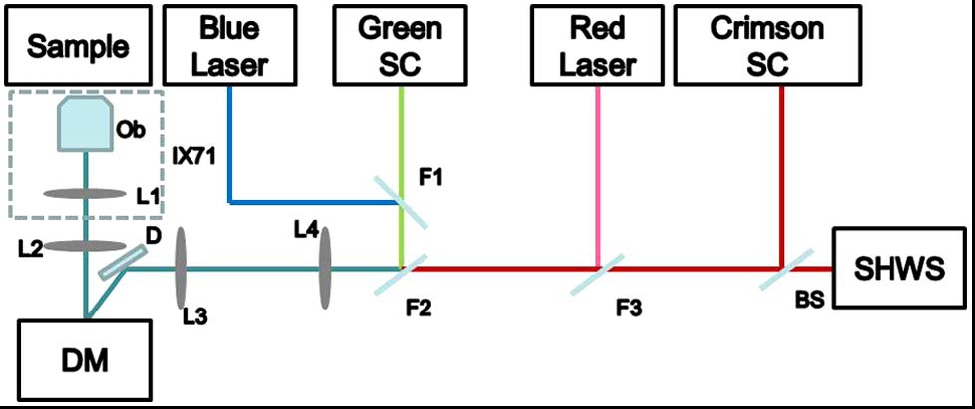
\includegraphics[width=0.60\textwidth]{images/Setup_widefield_direct.JPG}
		\caption{AO fluorescence microscope setup. The blue laser and the green camera correspond to the imaging channel of the sample. The red laser and the crimson camera correspond to measurement and correction channel. Image after \cite{wide_directSensing_microscope}.}
	\label{fig:Setup_widefield_direct}
\end{figure}


The final data analysis of \emph{Azucena et al.}  demonstrated that their approach can improve the resolution for an image gathered at 510 nm even though the wavefront measurement and correction is made at 647 nm (Fig. \ref{fig:wide_direct_results}). This is due to the fact that the wavefront sensor measures the change in optical path difference, which does not vary significantly over a large portion of the visible spectrum \cite{wide_directSensing_microscope}.

\begin{figure}[htbp]
	\centering
		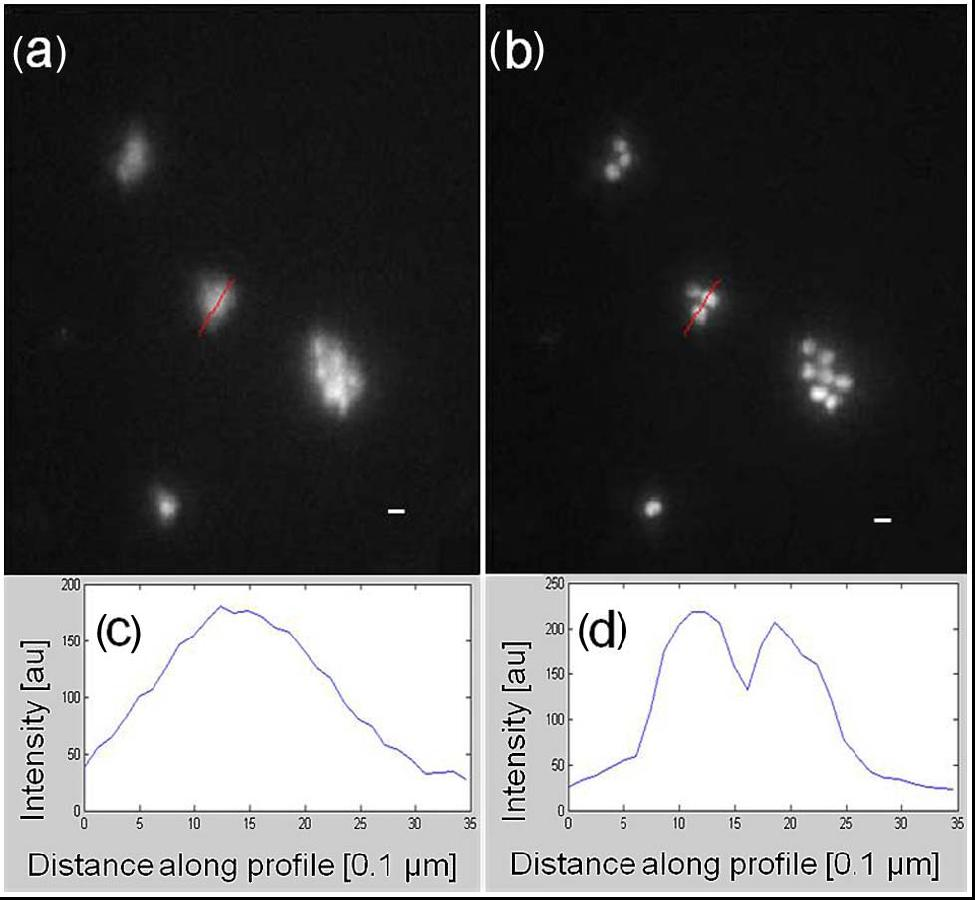
\includegraphics[width=0.40\textwidth]{images/wide_direct_results.JPG}
		\caption{Microspheres imaging. In (a) with AO system off, in (b) with AO system on. In (c) intensity profile of red line showed in (a). In (d) intensity profile of red line showed in (b). The white line is approximately ($\unit[1]{\upmu m}$ in length. Image after \cite{wide_directSensing_microscope}.}
	\label{fig:wide_direct_results}
\end{figure}


%------------------------------------------------------------------------------
\subsubsection{Indirect Wavefront Sensing in a Transmission Microscope}
\label{sec:TransmissionMicroscope}

To implement adaptive optics with standard (incoherent) transmission microscopes, \emph{Debarre et al.}~\cite{wide_AOM_loew_freq} implemented an indirect, sensorless and image-based adaptive optics scheme. As described earlier in Section~\ref{sec:IndirectWavefrontSensing}, image-based techniques do not require an additional wavefront sensor but retrieve the correction data directly form the recorded images. Hence the authors used a standard microscope for AOM by simple adding a deformable mirror in the beam path~(see ~\cite{wide_AOM_loew_freq} for experimental setup). As with all indirect sensing schemes, the difficulty is to find a good metric for image quality, which allows to determine the appropriate correction parameters. The presented method uses low spatial frequency content of the image as the optimization metric. The aberration is represented in terms of Lukosz modes which are based on Zernike polynomials. The presented technique consists on modeling the effects of aberrations on the imaging of low spatial frequencies, which Lukosz modes are found to be ideal for. By modeling the aberrations as a series of Lukosz modes they develop an optimization metric as the sum of a range of low spatial frequencies. The optimization function is related to the coefficients of the aberration expansion by a Lorentzian function. The aberration correction process is then performed as the maximization of the Lorentzian. Due to its paraboloidal maximum, the use of simple maximization algorithms is possible. Furthermore, the authors show that the optimization can be performed as a sequence of independent maximizations for each aberration coefficient.

\begin{figure}[tbh]
			\centering
			\begin{subfigure}[b]{0.7\textwidth}
							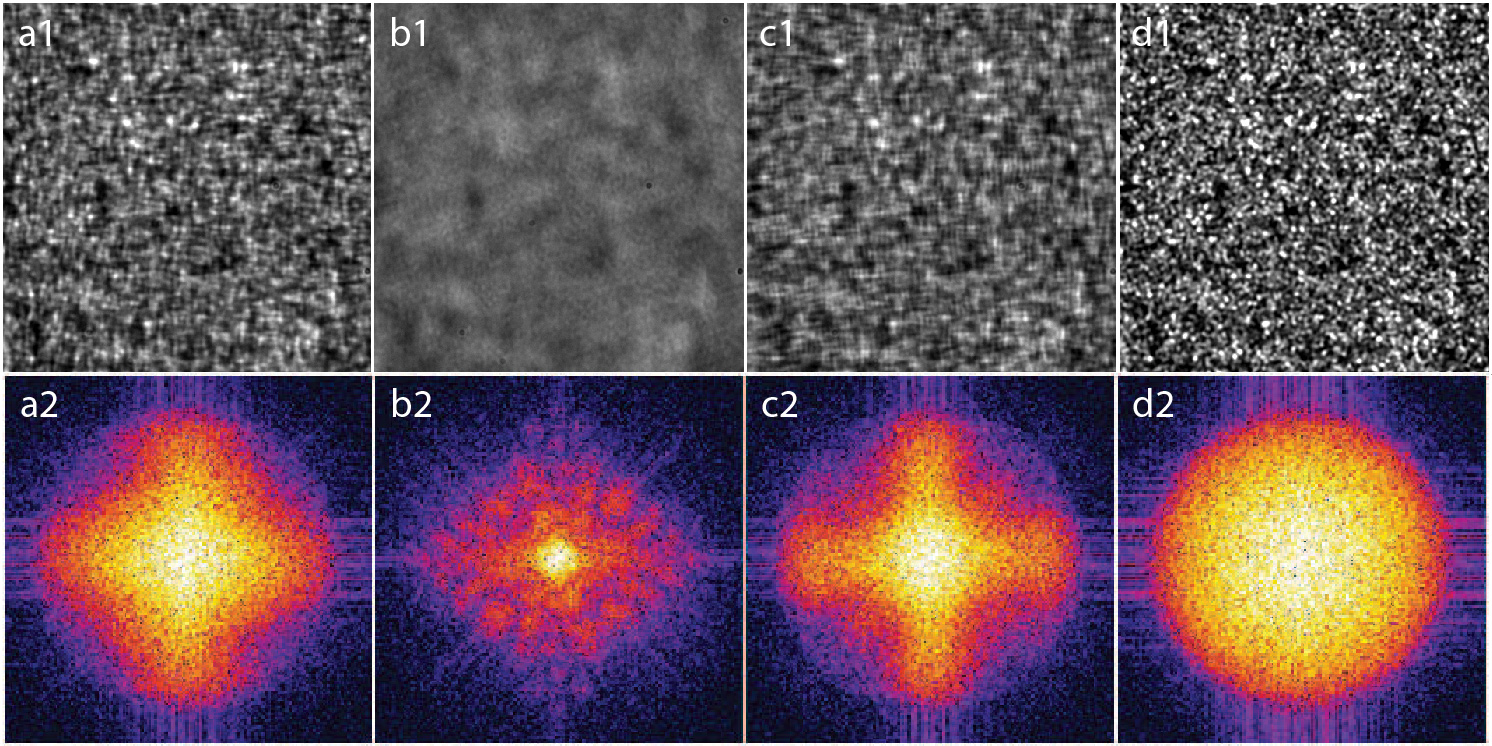
\includegraphics[width=\textwidth]{images/wide_parabolic_opti_images}
							\label{fig:para_opt_images}
			\end{subfigure}
			\begin{subfigure}[b]{0.7\textwidth}
							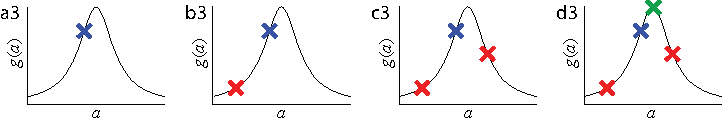
\includegraphics[width=\textwidth]{images/wide_parabolic_opti_graphs}
							\label{fig:para_opt_graphs}
			\end{subfigure}								
			\caption{Correction of a single Lukosz aberration mode (astigmatism, i = 5) for a scatterer specimen and using low spatial frequencies. The first row shows the raw images of the specimen and the second row illustrates schematically the sampling of the Lorentzian curve used in the optimization calculation. (a1~\&~a2) correspond to an arbitrary initial aberration of magnitude, (b1~\&~b2) have an additional negative bias while (c1~\&~c2) have an additional positive bias of equal magnitude. (d1~\&~d2) show the corrected image calculated with the parabolic minimization. Image after~\cite{wide_AOM_loew_freq}.}
	\label{fig:para_opt}
\end{figure} 

The correction process is shown in Figure~\ref{fig:para_opt} for the correction of a single Lukosz mode using a scatterer specimen. Using the deformable mirror (DM), an initial aberration is applied and an image is recorded. The Fourier transform and spectral density of the image are then calculated and the appropriate range of frequency components are summed, giving the metric measurements. The same procedure is repeated with both negative and positive aberrations~(i.e. stronger and weaker aberrations), resulting in two additional metric measurements, indicated by the red and blue crosses in Figure~\ref{fig:para_opt}~a2, b2, and c2. Due to the parabolic maximum of the Lorentzian, the maximum can be calculated from as little as three measurements~(indicated by the green cross in Fig.~\ref{fig:para_opt}~d2 and the correction is then applied to the DM. To correct multiple modes, each modal coefficient is measured in the same manner before the full correction aberration containing all modes is applied. While this technique is based only on low spatial frequencies, it is shown that both low and high frequency components can be effectively corrected. In all the cases investigated, a Strehl ratio greater than 0.8, close to the diffraction limit, was obtained. This indicates that, when aberration statistics are unknown, choosing small spatial frequencies for an initial correction is a reasonable strategy. If further correction is required, they can be performed using a larger range of frequencies. \emph{Debarre et al.} concluded that this correction scheme is largely independent of the object structure and proposed this approach also to be valid for coherent or partially coherent systems.

%------------------------------------------------------------------------------
\subsubsection{Structured Illumination Microscopy}
\label{sec:StructuredIlluminationMicroscopy}

It is often desired for biological samples to produce clear images of focal planes deep within a thick sample (i.e. optical sectioning) and common techniques include point-scanning techniques such as confocal or multiphoton techniques which are described in section~\ref{sec:PointScanningMicroscopes}. 

Widefield techniques such as Structured Illumination (SI) microscopy can also provide optical sectioning. However, the sectioning is realized using a standard microscopes, an incoherent light source and without the need for a scanning mechanism. For SI microscopy, a grid is imaged into the specimen to produce a one-dimensional sinusoidal excitation pattern in the focal plane. The resulting sinusoidal fluorescence image, consisting of both in- focus and out-of-focus fluorescence emission, is then normally recorded. Several images are taken, each corresponding to a different grid position equivalent to three different phase shifts of the grating. The grid pattern only appears in the focal plane while it is blurred in the out of focus regions. Hence, it is possible to extract an optical section from the spatially modulated component of the images via a simple calculation.

Based on the SI microscopy technique presented by \emph{Neil et al.} in 2005~\cite{wide_structured_illu_principle} as well as their earlier work on indirect wavefront sensing using a conventional microscope~\cite{wide_AOM_loew_freq} in 2007~(described in the previous section), \emph{Debarre et al.} combined both techniques in 2008 and proposed an AO scheme for use in SI microscopy~\cite{wide_AOM_structured_illu}.  

\begin{figure}[hbt]
	\centering
		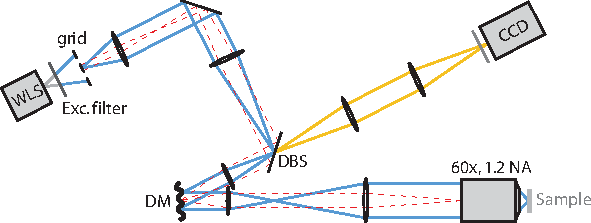
\includegraphics[width=0.75\textwidth]{images/wide_structured_illumination.pdf}
	\caption{Experimental setup for structured illumination microscopy with 
aberration correction. WLS~-~white light source, DM~-~deformable mirror, DBS
~-~dichroic beamsplitter. The blue rays mark the illumination path; the 
detection path is shown in yellow. Image after~\cite{wide_AOM_structured_illu}
.}
	\label{fig:wide_structured_illumination}
\end{figure}

They again presented a sensorless wavefront detection scheme, which is shown in Fig.~\ref{fig:wide_structured_illumination}. The method to obtain the aberration correction is similar to the one presented and explained in the previous section, and will not be described again. The results of the implemented AO scheme is shown in Fig.~\ref{fig:structured_light_correction} for aberration correction on a fluorescent mouse intestine. The image contrast and sharpness improvement is clearly visible in the image~\ref{fig:SI_corrected} compared to the uncorrected image in \ref{fig:SI_uncorrected}. As a result of the aberration correction, and as shown in Fig.~\ref{fig:SI_scan}, the contrast of small sample features (blue arrows) is better defined after (red solid line) rather than before (black dotted line) correction. 

\begin{figure}[htb]
        \centering
        \begin{subfigure}[b]{0.25\textwidth}
                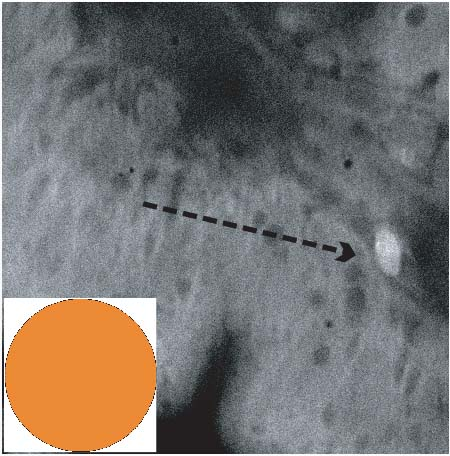
\includegraphics[width=\textwidth]{images/structured_illumination_uncorrected}
                \caption{Uncorrected.}
                \label{fig:SI_uncorrected}
        \end{subfigure}
        \begin{subfigure}[b]{0.25\textwidth}
                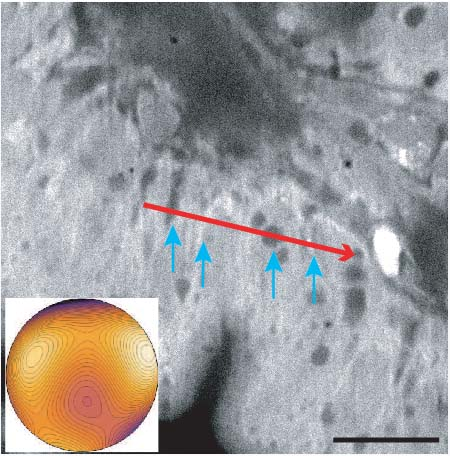
\includegraphics[width=\textwidth]{images/structured_illumination_corrected}
                \caption{Corrected.}
                \label{fig:SI_corrected}
        \end{subfigure}
        \begin{subfigure}[b]{0.25\textwidth}
                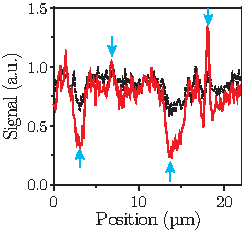
\includegraphics[width=\textwidth]{images/structured_illumination_scan}
                \caption{Line Scan.}
                \label{fig:SI_scan}
        \end{subfigure}
								
        \caption{Aberration correction in structured illumination microscopy. A fluorescent mouse intestine sample was imaged (a) without, (b) with aberration correction with inserts showing the phase induced by the deformable mirror. (c) Profile along the lines drawn on the images, both profiles normalized so that their mean value is identical. As a result of the resolution improvement, the contrast of small sample features (blue arrows) is better defined after (red solid line) rather than before (black dotted line) correction. The imaging depth was approximately $\unit[10]{\upmu m}$, sacle bar size $\unit[10]{\upmu m}$. Image after~\cite{wide_AOM_structured_illu}.}
\label{fig:structured_light_correction}
\end{figure} 

The authors also explained an additional benefit of aberration correction for structured illumination microscopy. The adaptive element can also be used to improve the rejection of the out-of-focus fluorescence. When imaging thick specimen, noise fluctuations in the fluorescence signal between the three successive widefield images obtained for the maximization process result in a large out-of-focus background in the calculated sectioned images. Since this background arises from fluorescence generated outside the focal plane, it is not sensitive to the presence of aberrations. By applying large aberrations the grid pattern is suppressed and only the out-of-focus noise can be measured. By subtracting this aberrated image from the original sectioned image, the fluorescent background can be efficiently removed, leading to greatly improved contrast of the in-focus structures. 

In conclusion, the authors presented a sophisticated, easy to implement and highly versatile AOM scheme which allowed for aberration correction induced by the optical system, the specimen or the focus depth. While the presented scheme used a widefield microscope, \emph{Debarre et al.} were also optimistic that similar AO methods based on indirect, image based aberration detection could be applied to point-scanning methods. 

%------------------------------------------------------------------------------
\subsection{Point Scanning Microscopes}
\label{sec:PointScanningMicroscopes}

Just as with the widefield techniques, adaptive optics quickly found its way into point scanning techniques to improve the image and signal quality. Scanning methods are useful for imaging biological specimens, since they can provide high resolution imaging in three-dimensions. Illumination is usually provided by a laser that is focused into the sample. The light emitted or reflected from the specimen is collected, usually through the same objective lens, and its intensity is measured by a detector. Since this only provides information about the intensity at a single spot, the focal point is then scanned through the specimen and point-by-point the image is acquired. 

This section will give a brief description how AO is applied to HG, CARS and STED microscopy. Following this will be a more detailed analysis of how adaptive optics is implemented into confocal~(section~\ref{sec:ConfocalMicroscopes}) and multi-photon florescence microscopes~(section~\ref{sec:MultiphotonScanningMicroscopyUsingIndirektSensing} and \ref{sec:TPFMDirect}). 

Adaptive optics techniques have been developed for all common point scanning microscopes. Using both the second- and third-harmonic intensity signals as the optimization metric for an indirect wavefront sensing scheme, \emph{Jesacher et al.}~\cite{scan_HG_dynamic} as well as \emph{Olivier et al}~\cite{scan_HG_embryos} showed AO applied to higher harmonic generation microscopy. The aberration correction is compensating both system- and specimen-induced aberrations when imaging live mouse embryos.The authors demonstrated an improved signal level and resolution, with peak intensity increased by almost $\ unit[50]{\%}$ and the FWHM decreased by $\unit[14]{\%}$ to  $\unit[1.22]{\upmu m}$ compared with a value of $\unit[1.15]{\upmu m}$ for a non-aberrated system.

Even better results were reported by \emph{Wright et al.}~\cite{scan_CARS} when applying AO to CARS. The authors achieved a signal improvement by a factor of 3 for samples at a depth of $\unit[700]{\upmu m}$ and a factor of 6 for muscle tissue at a depth of $\unit[260]{\upmu m}$. Their completely random optimization typically converged after 3000 changes mirror shapes. With a mirror speed of up to 1 kHz this is sufficiently fast. The approach is well suited to CARS microscopy where photobleaching does not occur but is less applicable for other microscopy techniques. 

It is also possible to apply AO to Stimulated Emission Depletion~(STED) microscopy~(see~\cite{scan_STED_principle} for basic working principle of STED) as recently presented by \emph{Gould et al.}~\cite{scan_STED}, again employing an indirect sensing scheme. Using a phase mask, the authors both created the doughnut shape depletion beam and simultaneously implemented an aberration correction. Using an additional spatial light modulator, aberration correction is also implemented in the excitation beam. The correction in the depletion beam leads to a better resolution while the correction of the excitation beam path results in a stronger signal and less noise. Unlike many other indirect sensing methods, here the image brightness proved to be a poor quality metric due to the depletion. Hence the authors introduced a new metric that seeks to optimize both image brightness and image sharpness in a combined approach. The new approach worked successfully resulting in a \~5-fold increase in the peak signal as well as a \~3.2-fold improvement in resolution.

%------------------------------------------------------------------------------
\subsubsection{Confocal Microscopes}
\label{sec:ConfocalMicroscopes}

The confocal microscopy can operate in reflection or fluorescence mode. Both are a dual pass system, which means that both the illumination path and the emission path have to be corrected in an AO confocal microscope. The first attempt to apply AO in confocal microscopy was done by \textit{Martin J. Booth et al.}~\cite{scan_CFM}. They implemented indirect wavefront sensing to a confocal fluorescence microscope in a closed-loop way. Aberration measurement and correction was done sequentially. First a preset positive bias aberration was introduced by a deformable membrane mirror. An image was taken and all of its pixel values were summed and averaged to give the value of $W_1$. Then, it was added to the system the equivalent negative bias aberration, obtaining $W_2$. They had shown before that the value of the difference signal, W=$W_1$-$W_2$, is approximately proportional to the amount of the Zernike mode Zi present in the sample. They applied this procedure for several different Zernike modes, updating the mirror shape each time. A simple representation of the experimental set-up is shown in Fig.~\ref{fig:AOM_scan_CFM}.

\begin{figure}[htbp]
	\centering
		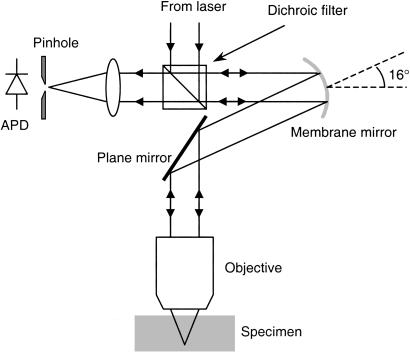
\includegraphics[width=0.42\textwidth,height=0.22\textheight]{images/AOM_scan_CFM.jpg}
		\caption{The illumination beam was passed through a beam expander and reflected by the membrane mirror such that the angle between the incident and reflected beams was 16º. Then it passed into the objective lens focusing the light into the specimen. Fluorescence light from the specimen was collected by the same objective. In this configuration, the membrane mirror can compensate for aberrations introduced into both the illumination and emission optical paths.}
	\label{fig:AOM_scan_CFM}
\end{figure}
  
With this sequential method for correcting aberrations they achieve a 1.8 times smaller axial PSF, using two cycles of this modal wavefront sensor applied to low order aberration modes.

A different way to apply AO in confocal microscopy was done by \textit{Xiaodong Tao et al} \cite{scan_Confocal_direct_sensing}. They used a direct wavefront sensor in a fluorescence confocal microscope. Particularly, they implemented a Shack-Hartmann sensor with fluorescent microspheres ($\unit[1]{\upmu m}$ diameter) embedded in the sample as a point source reference beacons. Their setup was designed to operate in a close-loop. The corrector device was a deformable mirror. A separate laser channel was added to excite the microsphere, which shared the same light path with the imaging channel. The results showed a $\unit[4.3]{\text{x}}$ improvement in the Strehl ratio and a $\unit[240]{\%}$ improvement in the signal intensity for fixed mouse tissues at depths of up to 100 $\mu$m. Although the effects of these microspheres in the live tissue have to be further investigated, this direct method enabled a shorter exposure time during sensing and a higher speed of imaging, which showed its potential ability for live in vivo imaging.


%------------------------------------------------------------------------------
\subsubsection{Indirect Wavefront Sensing in Multiphoton Scanning Microscopy}
\label{sec:MultiphotonScanningMicroscopyUsingIndirektSensing}

Its intrinsic optical sectioning, larger penetration depth, reduced photo damage as well as other advantages allowed nonlinear microscopy in general, and Two-Photon Fluorescence Microscopy~(TPFM) in particular, to become a very important tool in biological imaging since its first presentation by \emph{Denk et al.} in 1990~\cite{scan_TPFM_principle}. As with most AO microscopy techniques, both a direct and indirect wavefront sensing scheme can be deployed for the use with TPFM. Indirect sensing using a model based optimization was already explained~(section~\ref{sec:IndirectWavefrontSensing}) and presented~(section~\ref{sec:WidefieldMicroscopy} in detail. \emph{Marsh et al.} presented the first and fairly simple indirect sensing approach, correcting only for depth induced aberrations as early as 2003~\cite{scan_TPFM_pratical}. Again, based on their earlier works~(\cite{wide_AOM_loew_freq,wide_AOM_structured_illu}), \emph{D\'{e}barre et al.} presented another highly sophisticated application of their image based wavefront sensing scheme in 2009~\cite{scan_TPFM_image_based}. Since both \emph{Marsh} and \emph{D\'{e}barre} essentially used the standard TPFM setup and the image optimization is very similar to the one presented earlier, we will not describe these methods here again. \emph{Rueckel et al.} presented a wavefront correction method using coherence-gated wavefront sensing~\cite{scan_TPFM_gated_wavefront} which is beyond the scope of this report. 

For two-photon fluorescence microscopy, it is not essential to correct for sample or system induced aberrations on the collected beam. Since it is a point scanning technique, all the light emitted in the focus region is collected and only the relative intensity difference is important for the generation of the image~(see \cite{scan_TPFM_review} for a detailed review on TPFM). To achieve the highest possible resolution, especially when imaging deep in a tissue, it is however very important to correct aberrations of the excitation beam. This will not only result in a better, i.e. smaller focus spot, but will also highly increase the efficiency of the nonlinear process. As described in earlier sections, an indirect wavefront sensing is usually applied for microscopic applications, and such a system developed by \emph{Sherman et al.}~\cite{Genetic_MPFM} and based on a genetic optimization algorithm will be presented in this section. To overcome some of the inherent disadvantages of indirect sensing, \emph{Aviles-Espinosa et al.} developed a direct sensing scheme for two-photon fluorescence microscopy which will be described in section~\ref{sec:TPFMDirect}.

In multiphoton microscopy, the excitation of the sample by a high power, ultra short pulses is typically quadratic or cubic. If a diffraction limited spot is created in the focus of the laser beam, the generated nonlinear signal will have a maximum and hence signal intensity is a good image quality metric for these methods. Using a genetic optimization algorithm to maximize the nonlinear signal, \emph{Sherman et al.}~\cite{Genetic_MPFM} present a indirect sensing scheme for multiphoton microscopy correcting depth induced aberrations efficiently. Corrections were made with a genetic learning algorithm using the two-photon fluorescence intensity feedback to determine the desired shape for a deformable mirror. \emph{Albert et al.}~\cite{Genetic_smart_algorithm} were the first to investigate possible advantages of GA over random search algorithms in 2000. There, genetic algorithms were used for correcting off-axis aberrations in beam-scanning confocal microscopy, increasing the usable scan area by a factor of 9. Other adaptive optics methods using GA soon followed, optimizing fiber coupling efficiency~\cite{Genetic_fiber_coupling} or optimizing harmonic conversion efficiency~\cite{Genetic_Harmonic_optimization}. These methods however were not directly related to microscopy. It was \emph{Sherman et al.} who presented a better application of GA in microscopy, efficiently correcting for depth-induced spherical aberration and off-axis aberrations, providing full adaptive aberration compensation over a 3D volume. For simplicity, the authors used a Coumarin water solution in place of the biological sample that is commonly analyzed with multiphoton fluorescence microscopy. The long working distance objective allowed the scanning from the surface of the cover glass up to $\unit[2]{mm}$ into the sample. The aberration correction is achieved by running the genetic algorithm to determine the DM wavefront that would best maximize the two-photon intensity at the focus as measured by the fluorescence power. An optimum DM solution emerged after as little as 10 generations, resulting in a measurement time of approximately three minutes. This aberration correction can then be saved for future use, as long as the objective is the same and the location of the DM in relation to the microscope has not been changed. The first proof of an improvement in the image quality was done qualitatively by simply taking an image of the two-photon fluorescence as shown in Fig.~\ref{fig:genetic_TPFM_correction}. Since no biological sample is present, the imaged signal should ideally be a diffraction limited spot and hence the imaged points directly represent the lateral point spread function. The corrected image therefore shows a significant improvement in image quality.

\begin{figure}
	\centering
		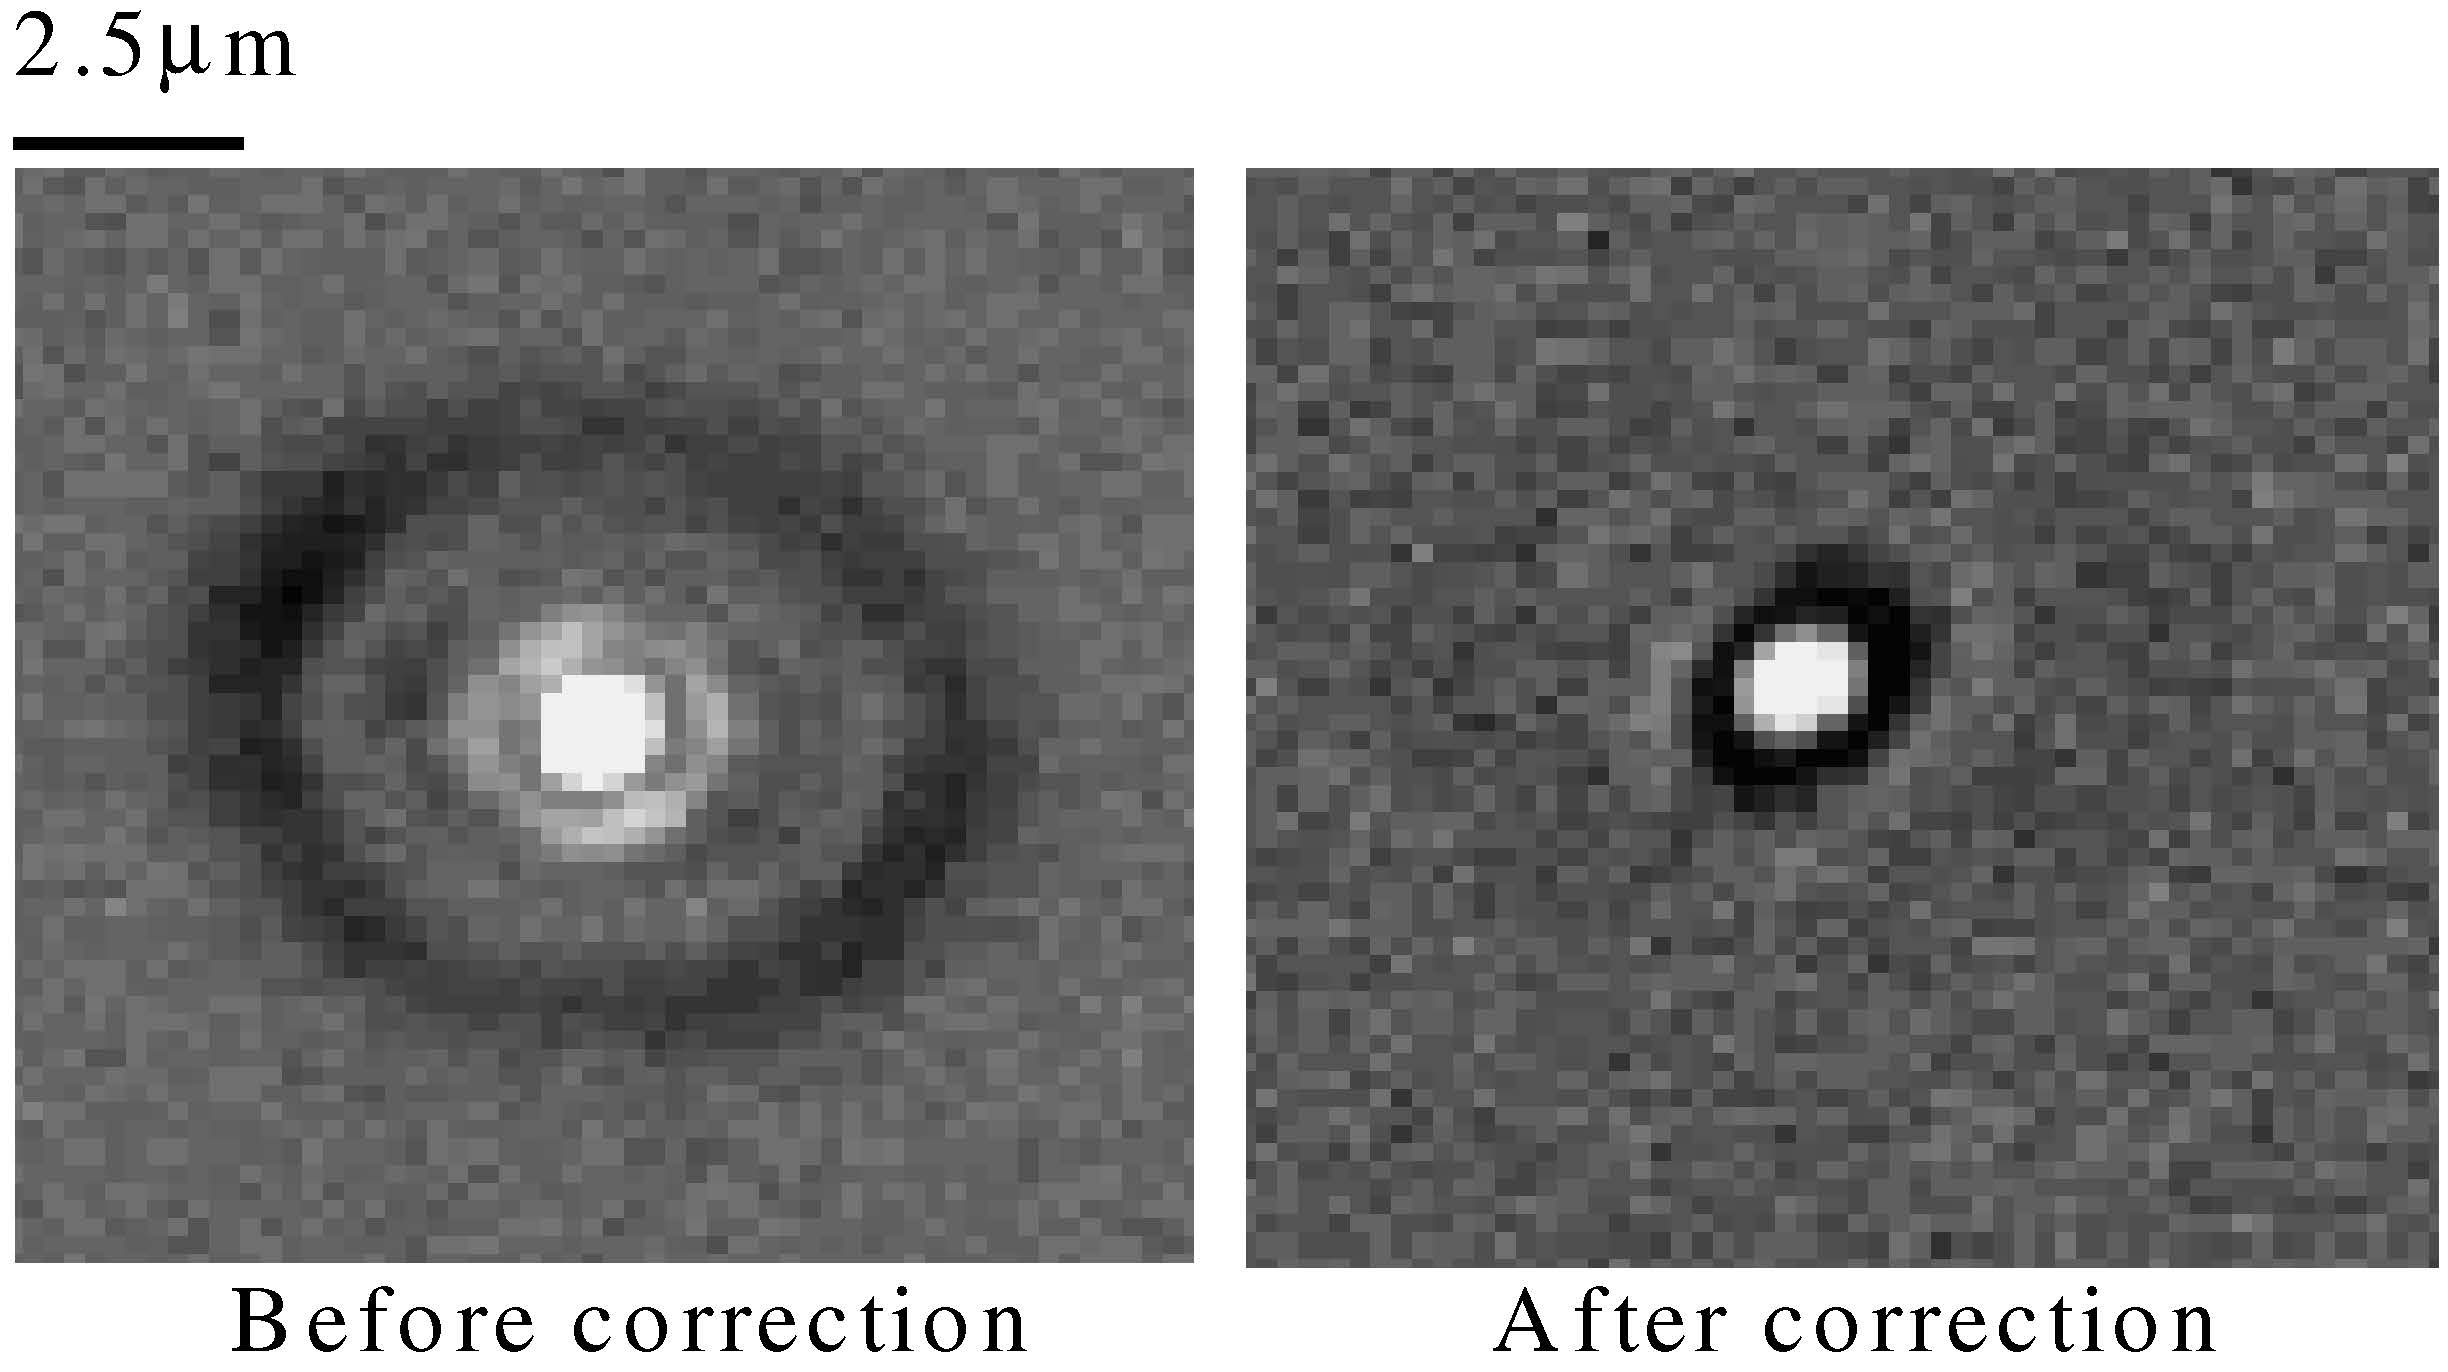
\includegraphics[width=0.50\textwidth]{images/genetic_TPFM_correction}
	\caption{Normalized CCD image of two-photon fluorescence at a focus depth of $\unit[600]{\upmu m}$ with and without correction with the DM.~\cite{Genetic_MPFM}}
	\label{fig:genetic_TPFM_correction}
\end{figure}

To quantify their results, \emph{Sherman et al.} scanned the laser focus spot along the longitudinal axis of a quartz/Coumarin-water interface. Third harmonic signals were generated at that interface and their signal intensity was used to measure the longitudinal PSF. The normalized longitudinal PSF as shown in Fig.~\ref{fig:genetic_TPFM_FWHM} reflects the normalized PSF decrease in FWHM from $\unit[14.6]{\upmu m}$ to $\unit[8.1]{\upmu m}$ with adaptive correction at a focus depth of $\unit[450]{\upmu m}$. The most significant result of correction is exemplified by the un-normalized longitudinal PSF shown in Fig.~\ref{fig:genetic_TPFM_intensity}. Whereas the normalized PSF shows the decrease in FWHM due to the combination of spherical bias and DM correction, in contrast to operation with no bias and no correction, the un-normalized longitudinal PSF shows a remarkable improvement in third harmonic intensity by a factor of more than 7 that results from compensating the spherical aberration.

\begin{figure}[tbh]
       \centering
        \begin{subfigure}[b]{0.45\textwidth}
                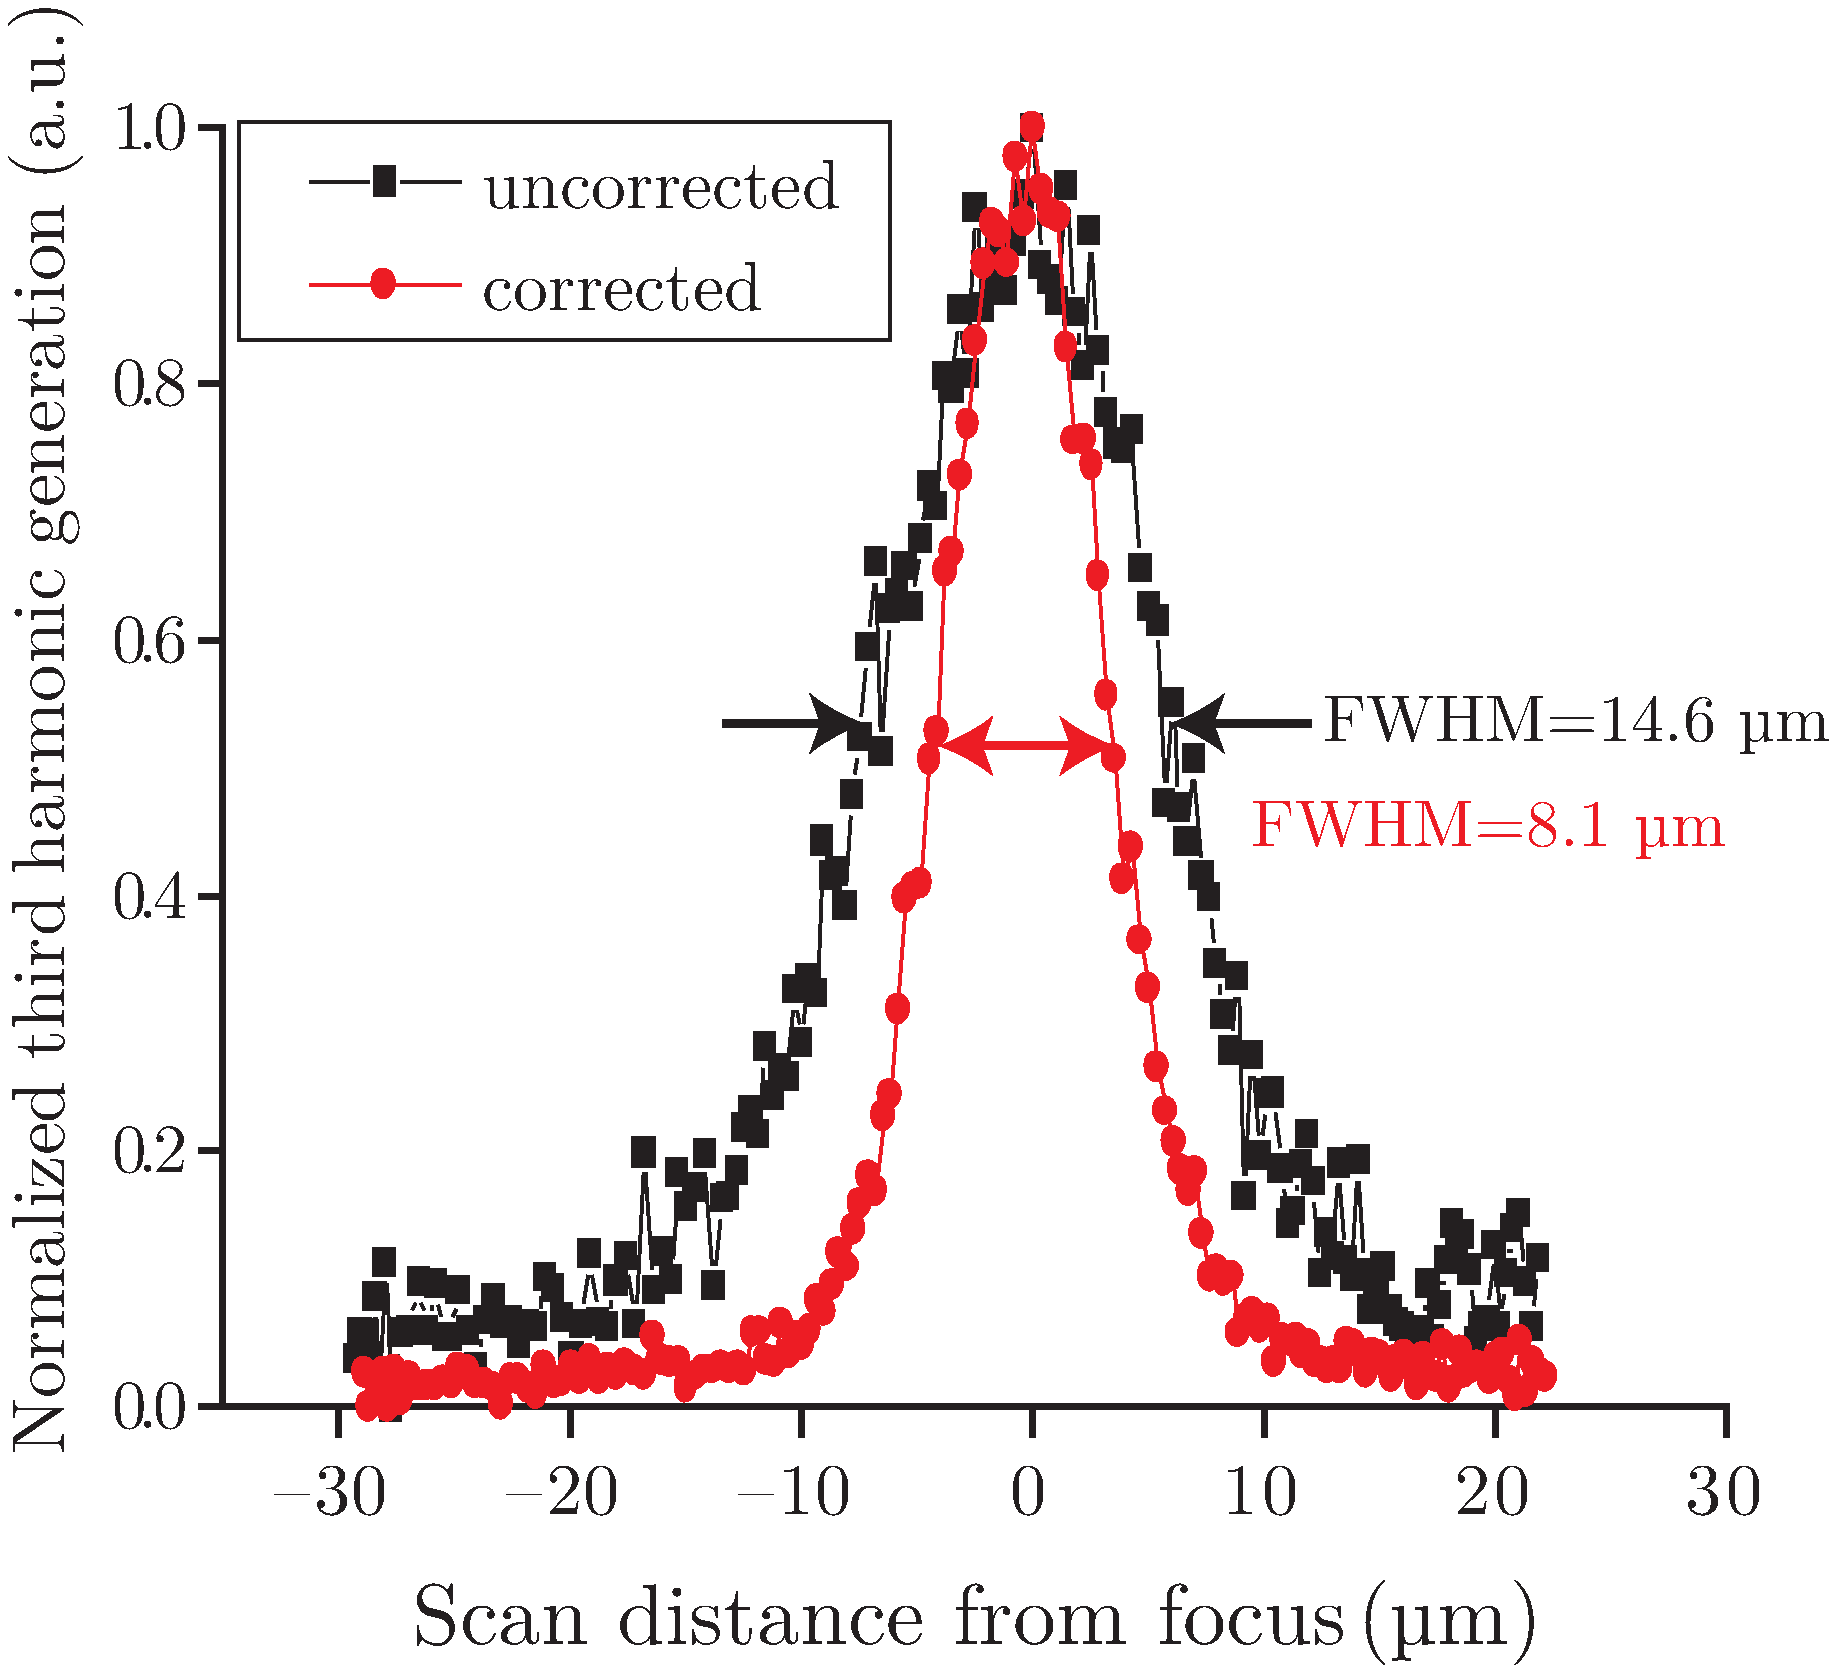
\includegraphics[width=\textwidth]{images/genetic_TPFM_FWHM}
                \caption{FWHM.}
                \label{fig:genetic_TPFM_FWHM}
        \end{subfigure}
				\hspace{1em}
        \begin{subfigure}[b]{0.45\textwidth}
                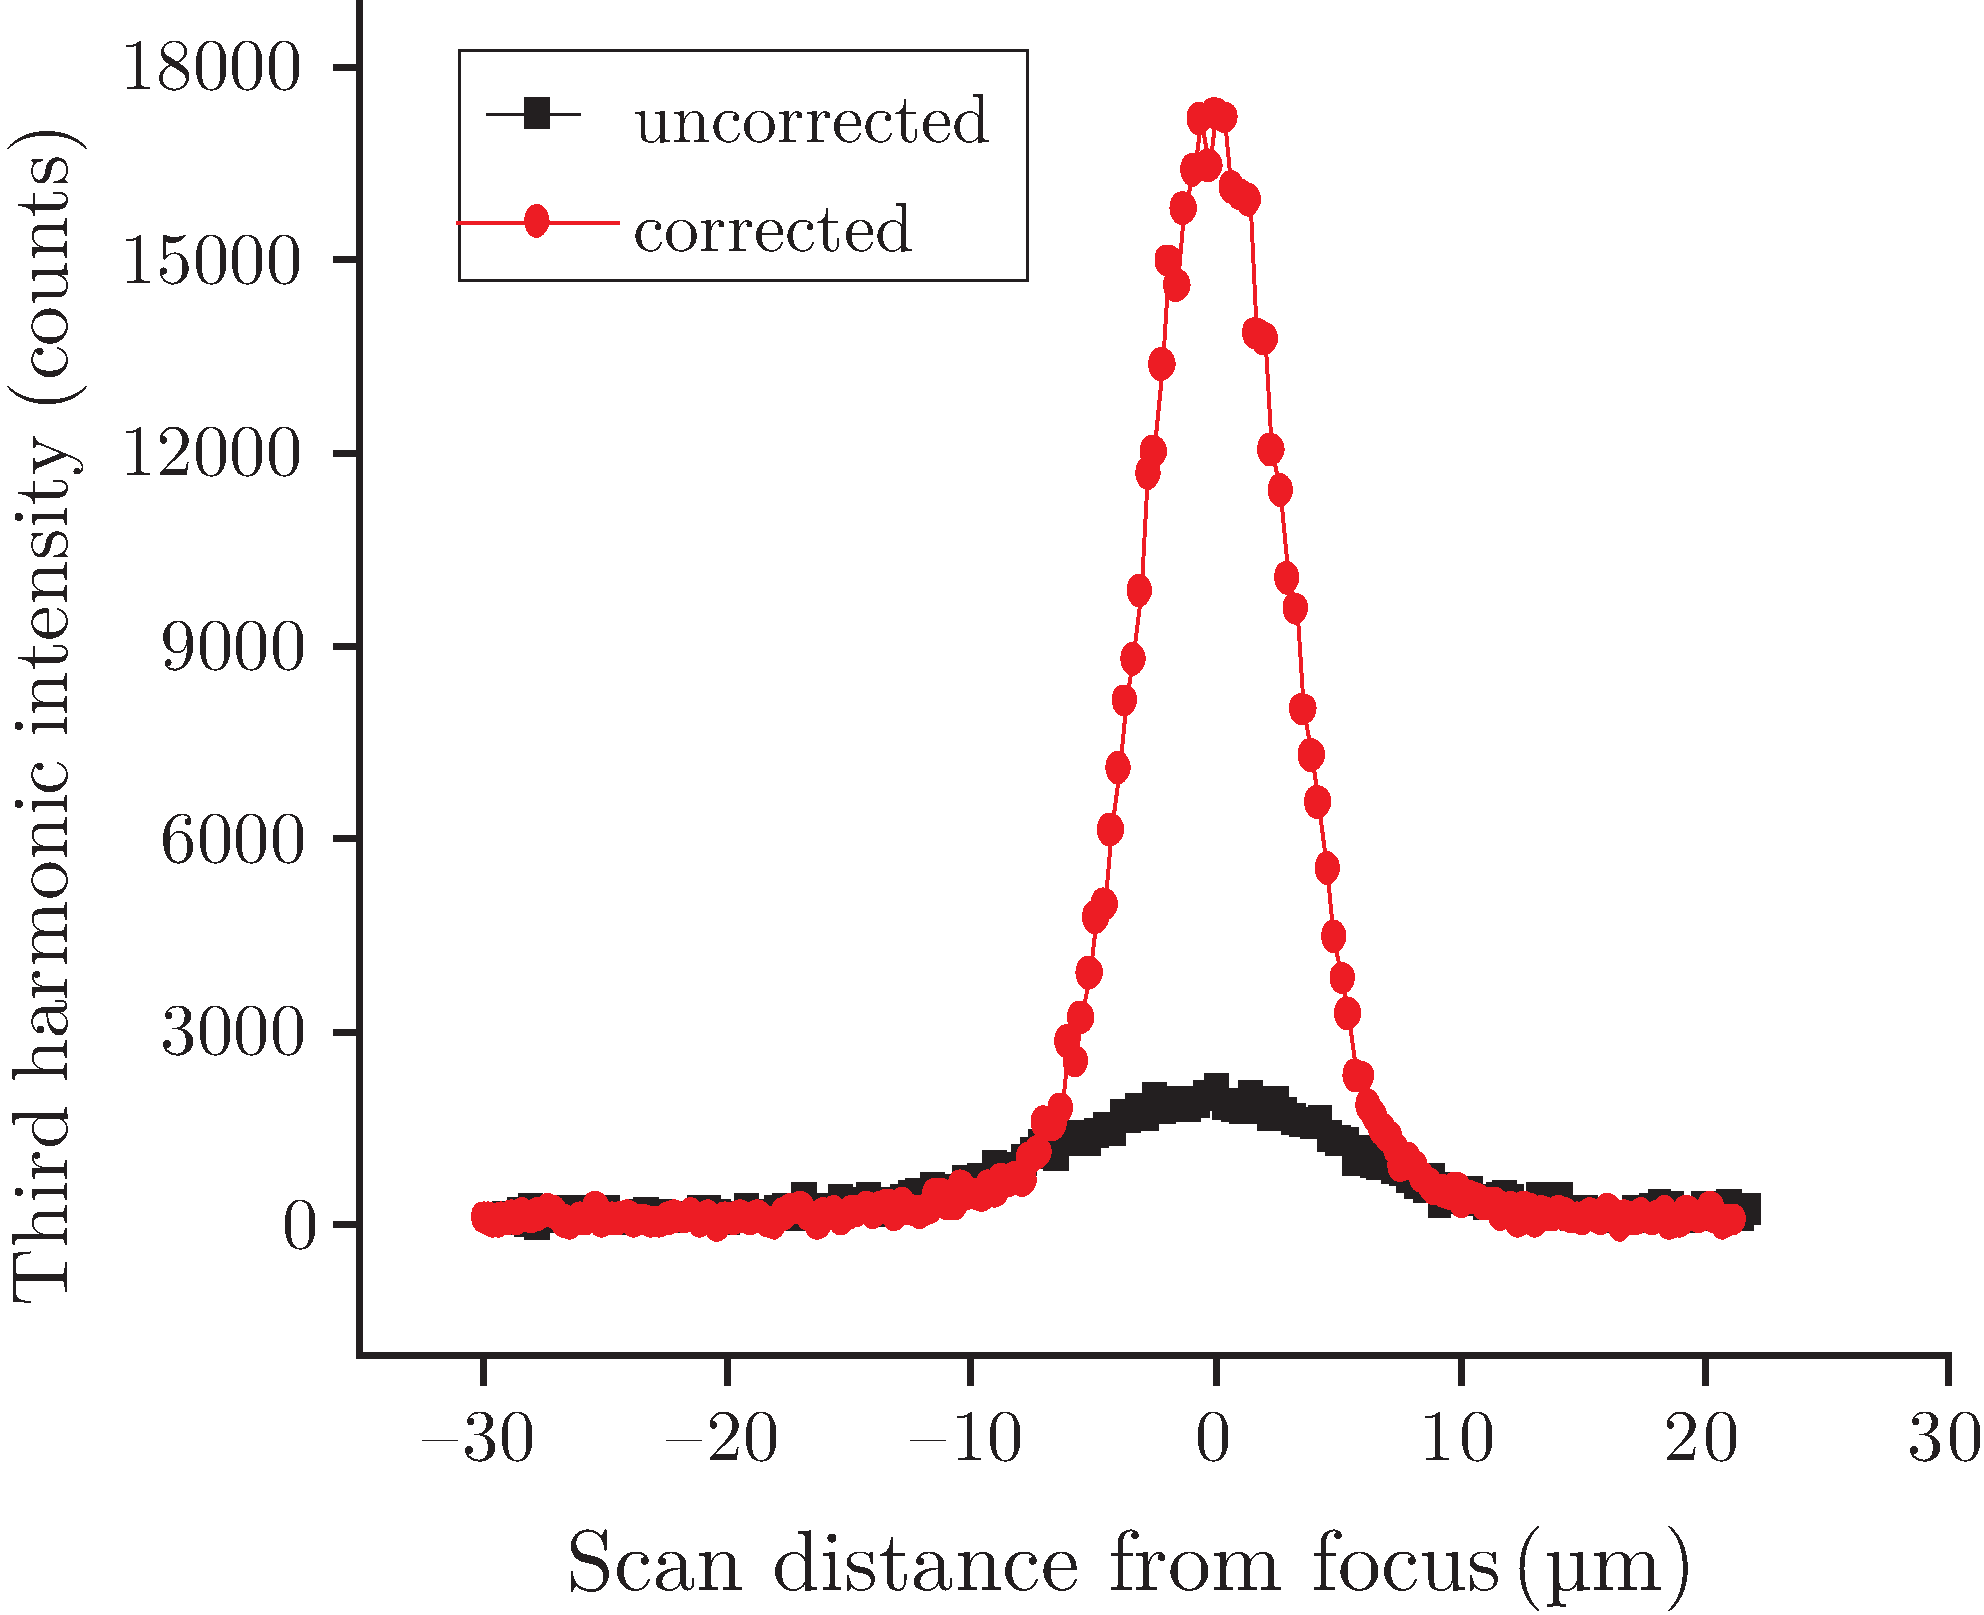
\includegraphics[width=\textwidth]{images/genetic_TPFM_intensity}
                \caption{Intensity.}
                \label{fig:genetic_TPFM_intensity}
        \end{subfigure}
        \caption{Normalized longitudinal point spread for focusing depth of 450 mm for both corrected and uncorrected showing increase in resolution due to correction, as well as un-normalized showing increase in intensity due to correction~\cite{Genetic_MPFM}.}
\label{fig:genetic_TPFM}
\end{figure} 

%------------------------------------------------------------------------------
\subsubsection{Direct Wavefront Sensing in Two Photon Florescence Microscopy}
\label{sec:TPFMDirect}

As described in section~\ref{sec:WavefrontSensing} and \ref{sec:DirectFluorescenceMicroscope}, to be able to use a wavefront sensor, one needs a point like reference source which is then used to detect the aberrations. This point like source can be artificially created and embedded in the sample. However, it might cause damage to the sample or might influence the behavior of living samples, limiting its potential for in vivo imaging. \emph{Aviles-Espinosa et al.} realized that two-photon excited fluorescence naturally produces a small confined volume that emits incoherently, thus it can be used as the guide-star. The setup presented by the authors is basically an inverted microscope, modified to be used as laser scanning TPFM (see paper for detailed component description and working principle). A mode locked Ti:sapphire laser~($\lambda = \unit[810]{nm}$ \& $\unit[860]{nm}$, pulse duration = $\unit[100]{fs}$, repetition rate = $\unit[80]{MHz}$, average powers in sample plane = $\unit[1.5]{mW}$ to $\unit[5.6]{mW}$) is used as the excitation beam. The wavefront sensing is performed using a Shack-Hartmann Wavefront Sensor (SH WFS), located at one of the output ports of the microscope. The aberration correction is realized with an electromagnetic Deformable Mirror (DM). The authors investigated the performance of their AOM system using both \emph{Caenorhabditis elegans} and mouse brain samples. For small aberrations and weak scattering only a modest improvement in signal intensity was shown. At an imaging depth of $\unit[25]{\upmu m}$, the measured signal enhancement was 1.75x by correcting the coupling aberrations, and 3.61x when focusing aberrations were corrected as well. Similar values were obtained imaging deeper into the tissue. \emph{Caenorhabditis elegans} tissue scatterers only weakly and hence spherical aberration is the main aberration for imaging deep into the tissue. Since these should be easily corrected using the presented scheme, the authors were surprised by these relatively small improvements in the signal quality. By using an additional agar pad to simulate moderate scattering as well as imaging deeper into the tissue, the authors investigated the correction efficiency further. Deep into the sample~($\unit[127]{\upmu m}$) where large sample induced aberrations are prominent, improvements of the signal intensity by a factor of 22.59 were possible, as shown in Fig.~\ref{fig:elegance}. It is noteworthy, that the aberration correction increases the signals local maxima while the local minima remain unaltered. 

\begin{figure}[tbh]
			\centering
			\begin{subfigure}[b]{0.20\textwidth}
							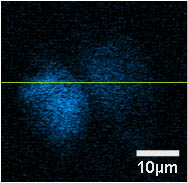
\includegraphics[width=\textwidth]{images/elegance_uncorrected}
							\caption{Uncorrected.}
							\label{fig:elegance_uncorrected}
			\end{subfigure}
			\begin{subfigure}[b]{0.20\textwidth}
							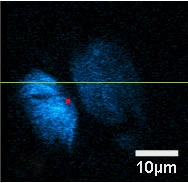
\includegraphics[width=\textwidth]{images/elegance_coupling_cor}
							\caption{Coupling cor.}
							\label{fig:elegance_coupling}
			\end{subfigure}		
			\begin{subfigure}[b]{0.20\textwidth}
							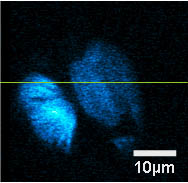
\includegraphics[width=\textwidth]{images/elegance_all_corr}
							\caption{Focusing cor.}
							\label{fig:elegance_all_corr}
			\end{subfigure}
			\begin{subfigure}[b]{0.37\textwidth}
							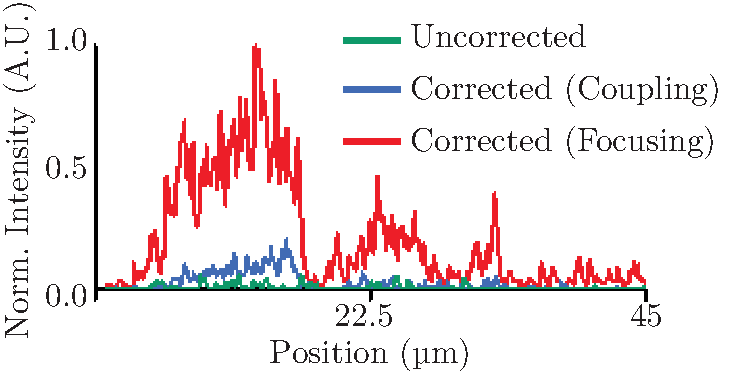
\includegraphics[width=\textwidth]{images/elegance_result}
							\caption{Line Scan.}
							\label{fig:elegance_result}
			\end{subfigure}							
			\caption{In vivo C. elegans sample imaged at $\unit[127]{\upmu m}$ depth. (a) shows the uncorrected image of a worm section, (b) displays the same section with coupling correction applied and (c) shows the section when both coupling and focusing aberrations are corrected. (d) shows the intensity profile along the green line in the images for all three correction cases. The correction of coupling aberrations improves the signal intensity by a factor of only 1.94 whereas the correction of both coupling and focusing aberrations results in a very good improvement of 22.59. Image after~\cite{scan_TPFM_guide_start}.}
	\label{fig:elegance}
\end{figure} 

Finally, the authors investigated the AO system performance using strongly scattering mouse brain tissue. They showed that a correction is still possible, but it is less efficient than for moderately scattering samples. It is furthermore possible to record aberration corrected images with a single exposure, no need for complex optimization algorithms and without further sample preparation~(i.e. no fluorescent microspheres need to be inserted). This minimize photobleaching effects, photo-toxicity and limits negative effects to the living sample. Since no model is needed to correct the aberrations, the method is robust and can be applied to fixed and in vivo biological samples. An overall intensity improvement of more than one order of magnitude was shown is some cases. In conclusion, the authors presented a flexible and versatile application of adaptive optics in microscopy which can be used in wide range biological imaging applications where a high resolution is required. 

